\documentclass[uplatex,12pt]{jsarticle}
\usepackage{listings}
\usepackage[dvipdfmx]{graphicx}
\usepackage{here}
\lstset{basicstyle=\small,style=myCustomMatlabStyle}

\title {Functional and logic programming lab 2nd report}
\date{}
\begin{document}
\author{Yoshiki Fujiwara, 05-191023}
\maketitle

\section{Q.1: Peano Arithmetic}

\subsection{An example operation}

\begin{lstlisting}[caption=test code]
add (S (S Z)) (S Z);; -> nat = S (S (S Z))

sub (S (S Z)) (S Z);; -> nat = S Z

sub (S Z) (S (S Z));; -> nat = Z

mul (S (S Z)) (S (S (S Z))) nat = S (S (S (S (S (S Z)))))

pow (S (S Z)) (S (S (S Z)));; -> nat = S (S (S (S (S (S (S (S Z)))))))

n2i (S (S Z));; -> int = 2

n2i Z;; -> int = 0

i2n 2;; -> nat = S (S Z)
\end{lstlisting}

\subsection{Discussion}
This code is about Peano arithmetic. Z means zero and S means successor function. Adding n is written as applying successor function n times. Subtracting n is written as removing S n times. Multiplication is written using the additional function. Also, the power function is written using multiplication.

\section{Q.2: DFS}

\subsection{An example operation}
\begin{lstlisting}[caption=test code]
pre_order(Node('a', Node('b', Node('d', Leaf, Leaf),
 Node('e', Leaf, Leaf)), Node('c', Leaf, Node('f',
 Node('g', Leaf, Leaf), Leaf))));;
 -> char list = ['a'; 'b'; 'd'; 'e'; 'c'; 'f'; 'g']

in_order(Node('a', Node('b', Node('d', Leaf, Leaf),
 Node('e', Leaf, Leaf)), Node('c', Leaf, Node('f',
 Node('g', Leaf, Leaf), Leaf))));;
 -> char list = ['d'; 'b'; 'e'; 'a'; 'c'; 'g'; 'f']

level_order (Node('a', Node('b', Node('d', Leaf, Leaf),
 Node('e', Leaf, Leaf)), Node('c', Leaf, Node('f',
 Node('g', Leaf, Leaf), Leaf))));;
 -> char list = ['a'; 'b'; 'c'; 'd'; 'e'; 'f'; 'g']
\end{lstlisting}

These test codes are applied to a tree like the below pictures

\vspace{12pt}
\subsection{Discussion}

\subsubsection{About code}
The written code is very simple. First, divide type 'a tree into three pieces and then put them together in the specific order. That is all I did.
\subsubsection{Application}

Pre-order outputs the node root as the first one. Then, it outputs left as the second one and right as the last one. Pre-order traversal is used in order to get a prefix expression of an expression tree.

In-order outputs the node left as the first, root as the second and right as the last. In-order traversal is used in case of a binary search tree. In-order traversal gives us the nodes in BST n non-decreasing order.

Post-order outputs the node left as the first, right as the second, and root as the last. Post-order traversal is used in order to delete the tree.

\begin{figure}[H]
 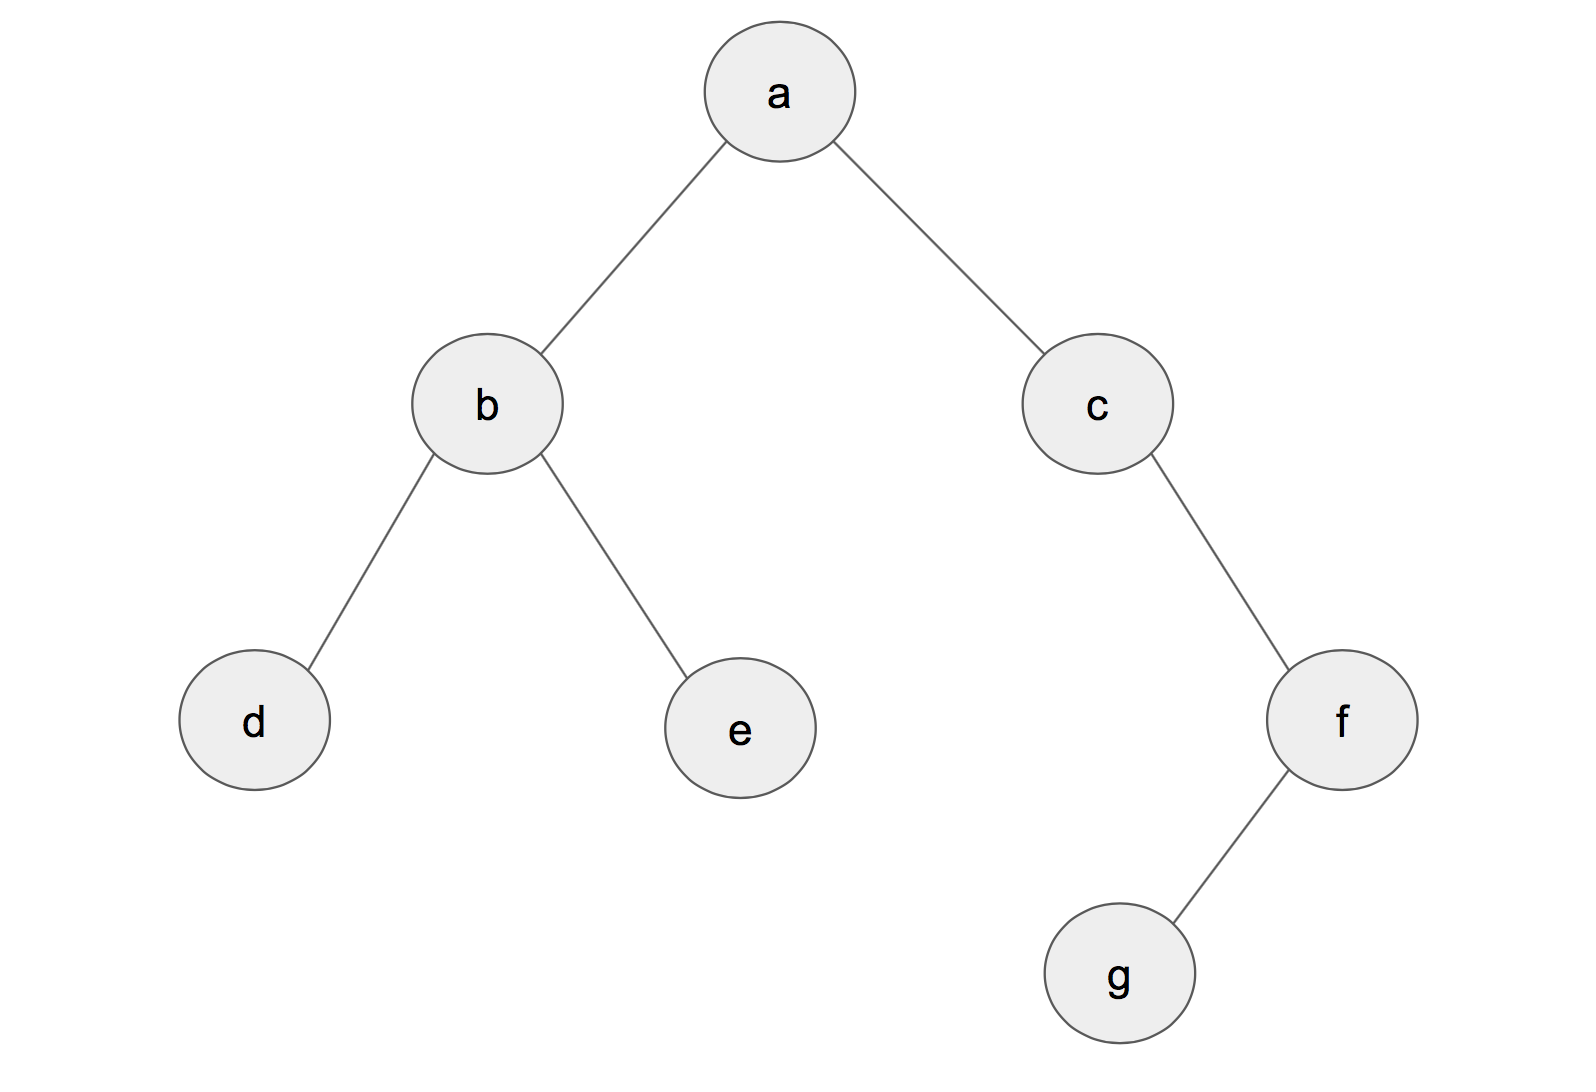
\includegraphics[scale=0.5] {binarytree.png}
 %\caption{binary-tree}
\end{figure}

\section{Q.3: BFS}

\subsection{An example of operation}
\begin{lstlisting}[caption=test code]
level_order (Node('a', Node('b', Node('d', Leaf, Leaf),
 Node('e', Leaf, Leaf)), Node('c', Leaf, Node('f',
 Node('g', Leaf, Leaf), Leaf))));;
 -> char list = ['a'; 'b'; 'c'; 'd'; 'e'; 'f'; 'g']
\end{lstlisting}

This example tree is the same as the above figure.
\vspace{12pt}
\subsection{Discussion}
\subsubsection{About code}
In the code, I created a list that stores type 'a tree. Recursion operates on the list as follows.
\begin{enumerate}
  \item Take an element 'a tree, from the list.
  \item If the element is a node, then memorizes the node in the accumulator.
  \item Then, push two subtrees (left and right) into the bottom of the list.
  \item Run 1. - 3. again and again until a node becomes Leaf.
\end{enumerate}

\subsubsection{Application and comparison with Q.2}
BFS is used in many ways, for example, to find the shortest path and to compute the maximum flow. DFS is easier to write than BFS because there is no need to make a list that stores subtrees. DFS is more compatible with functional programming.


\section{Q.4 and Q.5}
\subsection{An example of operation}

\begin{lstlisting}[caption=test code]
eval (Eif (EConstBool true, EConstInt 2, EConstInt 2));;
value = VInt 2
(* check "const", "bool" and "if"*)

eval (EAdd (EConstInt 2, EConstInt 2));;
value = VInt 4
(* check "EAdd"*)

eval (ESub (EConstInt 2, EConstInt 2));;
value = VInt 0
(* check ESub *)

eval (EMul (EConstInt 9,  EConstInt 3));
value = VInt 27
(* check EMul *)


eval (EDiv (EConstInt 9,  EConstInt 3));;
value = VInt 3
(* check EDiv *)

eval (Eeq (EConstInt 9, EConstInt 9));;
value = VBool true
(* check Eeq *)

eval (Ethan (EConstInt 9, EConstInt 3));;
value = VBool false
(* check Ethan *)

\end{lstlisting}


\vspace{12pt}
\subsection{Discussion}
The type of eval function must be "expr $\rightarrow$ value", OCaml's four arithmetic operations, like add function "+", are applied only to type int. Therefore we have to take apart type "expr" and pick out int type using "match" sentence. Plus, we need to raise an error if the improper codes are inputted.

\vspace{12pt}
optional 2(4) と3はできていません

\section{Q.6: fix funxtion}
\subsection{An example of operation}

\begin{lstlisting}[caption=test code]
type ('a, 'b) ty = NO | FIX of ((('a -> 'b) -> 'a -> 'b) -> 'a -> 'b)
exception Error
val fix : (('a -> 'b) -> 'a -> 'b) -> 'a -> 'b = <fun>
\end{lstlisting}

As above, I succeeded to define fix function without recursion.

\vspace{12pt}
\subsection{Discussion}
It is not easy to define the fix function without recursion. The key to solving this problem is to use type ref.

The basic idea of this problem is as follows.
\begin{lstlisting}[caption=basic idea]
let fix f x =
    let r = ref foo in
        let func g y =
                g (!r g) y in
                    (r := FIX func;
                    match !r with
                        !r f x);;
\end{lstlisting}

However, it is not the answer because the type is undecidable. We have to define a new type using variant.
\begin{lstlisting}[caption=type define]
type ('a, 'b) ty =
    | NO
    | FIX of ((('a -> 'b) -> 'a -> 'b) -> 'a -> 'b );;
\end{lstlisting}

Finally, we can define the fix function without recursion.


\section{Q.7: Curry-Howard}
\subsection{An example of operation}

\begin{lstlisting}[caption=output]
  type false_t = { t : 'a. 'a; }
  type 'a not_t = 'a -> false_t
  type ('a, 'b) and_t = 'a * 'b
  type ('a, 'b) or_t = L of 'a | R of 'b

  val q1 : ('a -> 'b) -> ('b -> 'c) -> 'a -> 'c = <fun>
  val q2 : ('a, 'b * 'c) or_t -> ('a, 'b) or_t * ('a, 'c) or_t = <fun>
  val q3 : ('a, 'b) or_t * ('a, 'c) or_t -> ('a, 'b * 'c) or_t = <fun>

  val callcc : (('a -> false_t) -> 'a) -> 'a = <fun>
  val q4 : ('a -> 'a) -> ('a not_t -> 'a) -> 'a = <fun>
  val q6 : ('a, 'a not_t) or_t -> (('a -> 'b) -> 'a) -> 'a = <fun>

\end{lstlisting}

\subsection{Discussion}
q1, q2, and q3 are written without recursion and reference like above.

q4 cannot be written without recursion and reference, because the law of the excluded middle cannot be proved in intuitionistic logic. However, using the callcc function enables us to connect intuitionistic logic and classical logic. It means q4 can be written using callcc.

q5 cannot be written, because this statement, $a \land \lnot a$, is always undefined.

q6 cannot be written without recursion and reference, because Perth's law cannot be proved without the law of excluded middle. We can define q7 using $a \lor \lnot a$ as above.

\section{Q.8: Curry uncurry}

未決定な単相を使うことでcurry uncurryの引数をずらそうとしたが失敗した。




\end {document}
